\documentclass[12pt]{article}
\usepackage[pdftex]{graphicx}
\usepackage[T1]{fontenc}
\usepackage{textcomp}
\usepackage{hyperref}
\hypersetup{
    colorlinks,
    citecolor=black,
    filecolor=black,
    linkcolor=black,
    urlcolor=cyan
}
\usepackage[text={16cm,24cm}]{geometry}
\usepackage{pgffor}
\usepackage{filecontents}% Used so that the external files can be placed in this file
%\setlength{\parskip}{\baselineskip}
\usepackage{color}
\definecolor{shadowgrey}{rgb}{0.18,0.2,0.21}
\usepackage{listings}
\lstset{ %
  frame=shadowbox,
  rulesepcolor=\color{shadowgrey},
  basicstyle=\footnotesize,
  commentstyle=\footnotesize
}

%header and footers
\usepackage{fancyhdr}
\pagestyle{fancy}
\fancyhead{}
\fancyfoot{}
\fancyhead[CO,CE]{\leftmark}
\fancyfoot[CO,CE]{EtherCAT Dextrous Hand User Manual}
\fancyfoot[RO, LE] {\thepage}
\fancyfoot[RE, LO] {
\includegraphics{images/hand-small.png}}

%custom commands
\newcommand{\todo}[1]{\colorbox{yellow}{\textbf{TODO: #1} fill this in!}}
\newcommand{\linuxtilde}{\raise.20ex\hbox{$\scriptstyle\mathtt{\sim}$}}
\newcommand{\link}[1]{\hyperref[sec:#1]{\textbf{section~\ref*{sec:#1}}}}
\newcommand{\betterhref}[2]{\href{#1}{#2}\footnote{url: #1}}

\title{\textbf{EtherCAT Dextrous Hand} \\
- User Manual -}
\author{Shadow Software team - software@shadowrobot.com}

\makeindex

\begin{document}
\begin{titlepage}

\maketitle
\vspace{5cm}
\begin{center}

\includegraphics{images/logo-shadowDB.png}
\end{center}
\end{titlepage}

\tableofcontents
\newpage

\section{Overview}
\label{sec:overview}

\par This user manual will get you started with using our EtherCAT hand or simulated robots. We'll guide you through installing the code in \link{install}, explain where to find things in \link{navigate} and show you some basic commands and code samples in \link{running-our-code}. This guide ends with some pointers to essential documentation you should read (\link{where-to-go}), and some troubleshooting tips (\link{what-do-if}). \\

\par You can find below a kinematics diagram of the Shadow Hand. The joint names are indicated on the diagram. As a convention, and because of the way the Hand is actuated, the joint 1 and 2 for the first finger, middle finger, ring finger and little finger are grouped in the joint 0: \texttt{FFJ0 = FFJ1 + FFJ2}, \texttt{MFJ0 = MFJ1 + MFJ2}, etc.

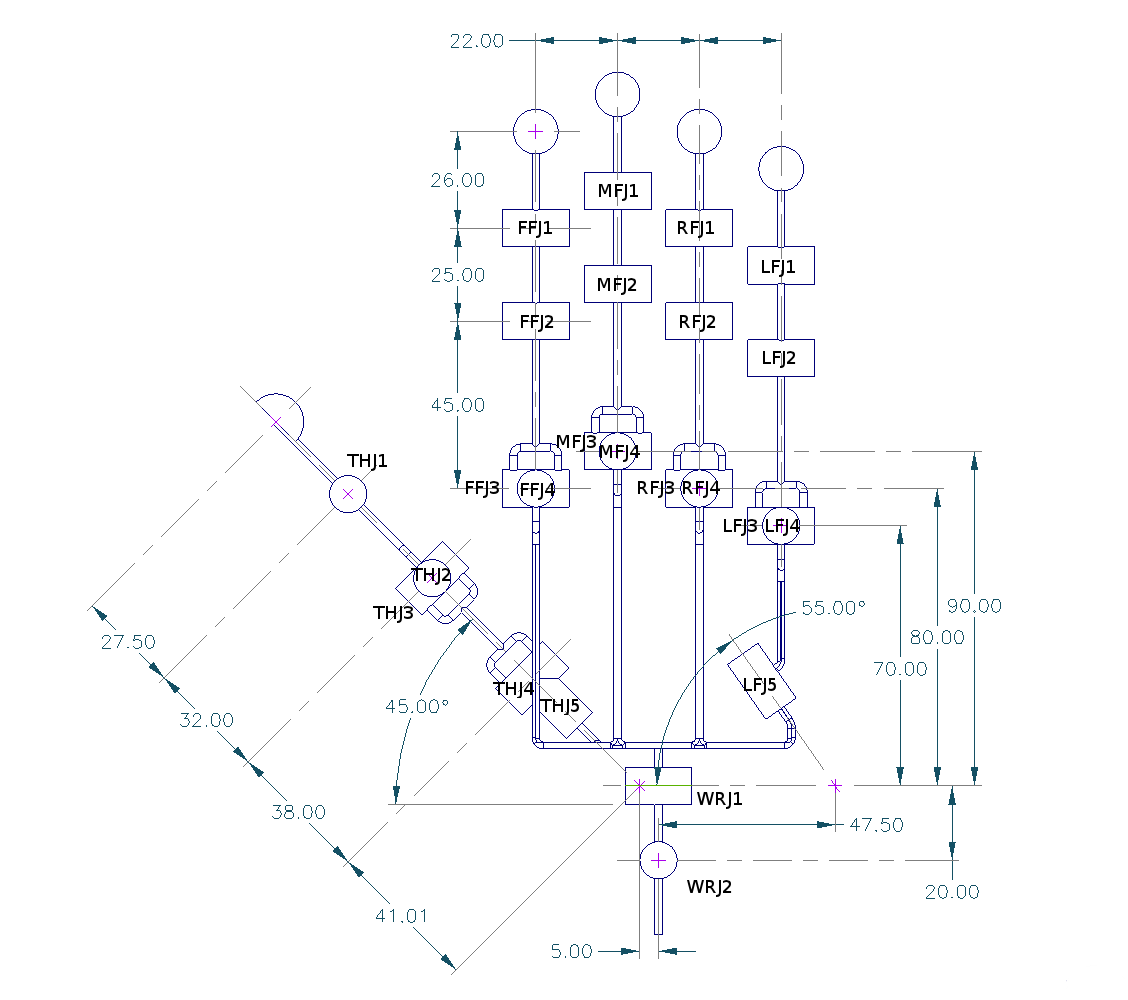
\includegraphics[width=\textwidth]{images/Hand_Kin_annotated.png}

\par If you have any questions, don't hesitate to contact us at: \texttt{software@shadowrobot.com}.\\

\newpage

\section{Installing our Software}
\label{sec:install}
\par For a typical user, we really recommend installing our software directly from the apt repository (see section \ref{sec:install-apt}). This will ensure that you keep the latest released software on your computer.\\

\par We assume you've already installed ROS Fuerte, as detailed on \betterhref{http://www.ros.org/wiki/fuerte/Installation/Ubuntu}{the ROS Wiki}.\\

\par However if you plan to modify some parts of our code, you can use an overlay\footnote{\textbf{Overlay:} use another version of a stack than the default installed one. The path to the package in the overlay will be prepended to the ROS\_PACKAGE\_PATH, so it will be used instead of the default installed version.} to install some of the sources from our publicly available Launchpad repository on top of your existing installation.

\subsection{From ROS apt repository (recommended)}
\label{sec:install-apt}
\par You can install pre-built packages for \betterhref{http://releases.ubuntu.com/precise/}{Ubuntu 12.04}. This is the easiest way of installing our software. You'll also receive updates automatically whenever you update your system.

Once you've installed ROS Fuerte, you can easily install our stacks:
  \begin{lstlisting}
> sudo apt-get install ros-fuerte-shadow-robot \
   ros-fuerte-shadow-robot-ethercat ros-fuerte-sr-visualization \
   ros-fuerte-sr-teleop
  \end{lstlisting}

\subsubsection{Install a sr\_config overlay for the EtherCAT Hand}
\label{sec:install-cfg}
\par If you have an EtherCAT Hand, you should create an overlay for the \texttt{sr\_config} stack: this stack contains all the different configuration files which can be modified to reflect your specific system. You shouldn't use the one installed by default as they are defined for the simulated hand.\\

\par To create this overlay, just follow \link{install-src}.

\subsection{From sources}
\label{sec:install-src}
\par If you need to modify one of the packages for your own use, you'll want to first install the released version from the apt repository as explained in \link{install-apt}. This will ensure that you have all the code you need. Once you've identified in which stack the package you want to modify is, you can create an overlay to use the source version.\\

\par To create an overlay, we'll use the \betterhref{http://ros.org/wiki/rosws}{rosws} utility. In this example, we'll overlay the \betterhref{http://launchpad.net/sr-config}{sr\_config} stack, using trunk version of the code hosted on launchpad using \betterhref{http://bazaar.canonical.com}{bzr}: \texttt{lp:sr-config}.

\begin{itemize}
\item First we need to install the rosws/rosinstall utilities if you haven't done so already (you've probably already installed this when following the ROS wiki instructions):
  \begin{lstlisting}[language=Bash]
> sudo apt-get install python-rosinstall python-rosdep bzr
  \end{lstlisting}

\item We're now going to create a workspace (in the \texttt{\linuxtilde/workspace} directory), based on your currently installed ROS system (we're assuming you're using ROS Fuerte), and add the stacks we want to overlay to the workspace. We'll then update the workspace to download the code into it.
  \begin{lstlisting}[escapeinside='']
> rosws init '\linuxtilde'/workspace /opt/ros/fuerte
> source '\linuxtilde'/workspace/setup.sh
> rosws set sr_config --bzr lp:sr-config
> rosws update
  \end{lstlisting}

\item To use the newly created environment, simply source the setup.sh created in the previous step (to have it sourced automatically when you open a new terminal, simply add it to your \texttt{\linuxtilde/.bashrc} as show on the second line).
  \begin{lstlisting}[escapeinside='']
> source '\linuxtilde'/workspace/setup.sh
> echo source '\linuxtilde'/workspace/setup.sh >> '\linuxtilde'/.bashrc
  \end{lstlisting}

\item Finally, you can build the whole stack in one go using the \texttt{rosmake} command:
  \begin{lstlisting}[escapeinside='']
> rosmake --rosdep-install --rosdep-yes sr_config
  \end{lstlisting}

\end{itemize}

\subsubsection{Available rosinstall files}
\par If you want to install all our stacks in one go, you can use the \texttt{rosinstall} files available \href{http://bazaar.launchpad.net/~shadowrobot/sr-build-tools/trunk/view/head:/data/shadow_robot-fuerte.rosinstall}{here}\footnote{url: http://bazaar.launchpad.net/\linuxtilde shadowrobot/sr-build-tools/trunk/view/head:/data/shadow\_robot-fuerte.rosinstall}.\\

\par Once you've downloaded the code using the \texttt{rosinstall} commands described previously, you can build all our stacks:
  \begin{lstlisting}[escapeinside='']
> rosmake --rosdep-install --rosdep-yes shadow_robot \
  shadow_robot_ethercat sr_contrib sr_visualization \
  sr_teleop
  \end{lstlisting}

\subsection{Import our custom Environment Variables}
\label{sec:import-vars}
\par As described in \link{spec-system-param}, we're using a file to define some useful environment variables. To make sure the variables are imported in your setup, you need to source it in your \texttt{\linuxtilde/.bashrc}, after sourcing the ros setup.sh. It should look like this:
  \begin{lstlisting}[title={\textbf{\linuxtilde/.bashrc}}, upquote=true]
#source the ros setup.sh
source /opt/ros/fuerte/setup.sh
#or the one created in your workspace
# if you used an overlay
#source ~/workspace/setup.sh

#now source our additional environment variables
source `rosstack find sr_config`/bashrc/env_variables.bashrc
  \end{lstlisting}

\newpage

\section{Navigating our code}
\label{sec:navigate}

\par Our code is splitted into different stacks, each containing a set of packages:
\begin{itemize}
\item \textbf{shadow\_robot:} contains simulation software, utility packages, ... This is the core stack.
\item \textbf{shadow\_robot\_ethercat:} contains the code for running our etherCAT hand.
\item \textbf{sr\_contrib:} contains experimental high level packages. If you write some interesting package, we'd be happy to add it to this stack.
\item \textbf{sr\_visualization:} contains the GUI and visualisation tools.
\item \textbf{sr\_teleop:} contains drivers for different tools used to teleoperate our hand (\betterhref{http://www.cyberglovesystems.com}{cyberglove}, ...)
\item \textbf{sr\_config:} contains the configuration files. If you have one of our Hand, you should have an overlay of this configuration to make sure you don't loose your configuration when updating your system (as described in \link{install-src}).
\end{itemize}

\subsection{Important Packages}
\label{sec:important-packages}
\begin{itemize}
\item \textbf{sr\_hand:} Contains the code and the different launch files for the simulated Hand and the CAN hand.
\item \textbf{sr\_edc\_launch:} Contains the main launch file for the EtherCAT Hand.
\item \textbf{sr\_example:} Contains some simple code examples.
\end{itemize}


\subsection{Where to find the settings}
\label{sec:where-find-settings}
\par We moved all the configuration to the \texttt{sr\_config} stack. The idea is to isolate the data that is specific to the user in a given stack, this way you can easily create an overlay, as described in \link{install}, to make sure your specific configuration is not overwritten by an update.

\subsubsection{Specifying system parameters}
\label{sec:spec-system-param}
\par The system parameters are specified in the file
\href{http://bazaar.launchpad.net/~shadowrobot/sr-config/trunk/view/head:/bashrc/env_variables.bashrc}{env\_variables.bashrc}\footnote{url: http://bazaar.launchpad.net/\linuxtilde shadowrobot/sr-config/trunk/view/head:/bashrc/env\_variables.bashrc}. To load them automatically in your environment, please go to \link{import-vars}. This File is heavily commented and should be easy to modify to suit your installation (the default options should be ok for most users).

  \begin{lstlisting}[title={\textbf{env\_variables.bashrc}}, upquote=true]
#set to 1 to compile sr_hand and sr_tactiles with the gazebo interface
export GAZEBO=1

# set to 1 for one finger hands
export ONE_FINGER=0

# set to 1 for left hands
export LEFT_HAND=0

# set to 1 if you have a CAN hand
export REAL_HAND=0

# set to 1 if you have a CAN arm
export REAL_ARM=0

#set to 1 if you have a muscle arm or hand
export VALVES=0

#set to 1 if you want to build compatibility interface for etherCAT hand
export ETHERCAT=0

#specify which port is used for the etherCAT hand
export ETHERCAT_PORT=eth1

#set to 1 if you're using PWM control on the etherCAT hand motors by default
export PWM_CONTROL=0

#set to 1 if you want to have access to the internal firmware repository
#NOTE: for Shadow employees only for the time being
export INTERNAL_FIRMWARE=0
  \end{lstlisting}


\subsubsection{Specifying default controllers settings, and other useful settings}
\label{sec:spec-defa-contr}
\par The controller settings (as well as the different mappings and polling rates for the etherCAT hand) can be found in the \textbf{sr\_ethercat\_hand\_config} package. You can modify the controller values which will be loaded by default by modifying the files in this package. For example if you want to modify the mixed position velocity controllers, you can open \textbf{sr\_edc\_mixed\_position\_velocity\_joint\_controllers.yaml} (in \textbf{controls/host}). We recommend using the controller tuner GUI plugin for tuning and saving those parameters.

\newpage

\section{Running our code}
\label{sec:running-our-code}

\subsection{Starting the real hand}
\label{sec:starting-real-hand}

\subsubsection{Setting up the Ethernet port}
\par The first time you plug an EtherCAT Hand, you probably need to check on which Ethernet port the hand is connected (you probably have 2 network ports in your computer, one of them would typically be connected to the network, the other one to the hand).\\

\par An easy way to see which port the hand is using is to unplug the hand network cable from your computer and then plug it back in. You can now type \texttt{dmesg} and you should see a line saying which port has just been plugged in, for example, in the lines below, you see that \texttt{eth1} is used by the hand:
  \begin{lstlisting}[escapeinside='']
[16661.901920] e1000e: eth1 NIC Link is Down
[16666.460518] e1000e: eth1 NIC Link is Up 1000 Mbps Full Duplex
  \end{lstlisting}

\par Now that we know which Ethernet port is used by the hand (\texttt{eth1} in our example), we can edit the interface in the system parameters, as shown in \link{spec-system-param}:
\begin{itemize}
\item Make sure you've created your overlay for the \texttt{sr\_config} stack as described in \link{install-cfg}.
\item Let's open the configuration file:
  \begin{lstlisting}[escapeinside='']
> roscd sr_config
> cd bashrc
> gedit env_variables.bashrc
  \end{lstlisting}
\item Set the \texttt{ETHERCAT\_PORT} to the correct value (it is \texttt{eth1} by default)
\item Save and restart your terminal to make sure the new options have been taken into account.
\end{itemize}

\subsubsection{Starting the driver}
\par You can now start the driver. To be able to run the driver, you need to elevate the permissions to root access:
  \begin{lstlisting}[escapeinside='']
#elevate permissions
> sudo -s
> roslaunch sr_edc_launch sr_edc.launch
  \end{lstlisting}

\subsection{Starting the simulated robot}
\label{sec:start-simul-hand}
\par To start the simulated robot you can simply run:
  \begin{lstlisting}[escapeinside='']
> roslaunch sr_hand gazebo_hand.launch
  \end{lstlisting}

\par Or if you want a simulated Shadow Arm as well as our hand:
  \begin{lstlisting}[escapeinside='']
> roslaunch sr_hand gazebo_arm_and_hand.launch
  \end{lstlisting}

\subsection{Starting the GUI}
\label{sec:start-gui}
\par We're using the \betterhref{http://www.ros.org/wiki/rqt\_gui}{rqt\_gui} for driving the hand. We implemented some plugins to help you control the hand. They are all in the Shadow Robot item in the plugins menu.

\par To start the GUI, you can simply run:
  \begin{lstlisting}[escapeinside='']
> rosrun rqt_gui rqt_gui
  \end{lstlisting}

\subsection{Checking it works}
\label{sec:checking-it-works}

\subsubsection{Reading data out of the Hand}
\par You can first have a look at the data coming out of the hand. The data is published on the \texttt{/joint\_states} topic (or \texttt{/gazebo/joint\_states} for the simulated hand). You'll see the incoming data streaming in your console. You have access to the joint names as well as the current positions (in radians), velocity (in radians per second) and effort (an arbitrary value, proportional to the effort applied at the motor-end of the tendon.) for each joint as shown below (stop with \texttt{ctrl+c}):
  \begin{lstlisting}[escapeinside='']
> rostopic echo /joint_states
---
header:
  seq: 7235
  stamp:
    secs: 73
    nsecs: 785000000
  frame_id: ''
name: ['WRJ2', 'WRJ1', 'FFJ4', 'FFJ3', 'FFJ1', 'FFJ2', ...]
position: [-0.007345193851005405, 0.0007282010249589632, ...]
velocity: [0.0002164649710794793, 0.0015999764385997265, ...]
effort: [0.0, 0.0, 0.0, 0.0, ...]
  \end{lstlisting}

\par You should also be able to visualise the current state of the robot using \betterhref{http://www.ros.org/wiki/rviz}{rviz}.
\begin{center}
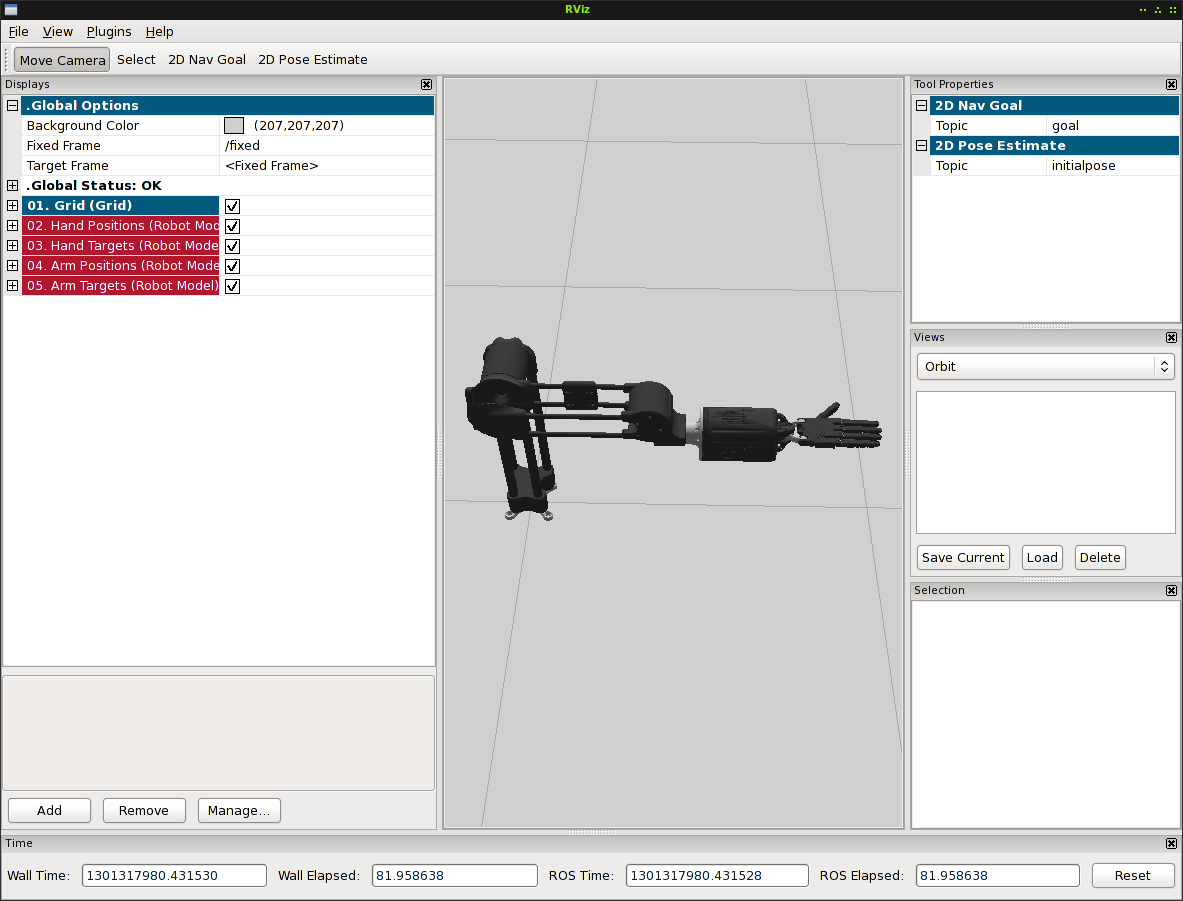
\includegraphics[width=0.5\textwidth]{images/rviz.png}
\end{center}

\subsubsection{Reading the tactile sensors}
\par Depending on the configuration of your hand, you can have different models of tactile sensors. Your sensor type is automatically detected by the driver which then publishes the correct information on \texttt{/tactile} topic. The following command will output the data coming from the sensors on the screen.
  \begin{lstlisting}[escapeinside='']
> rostopic echo /tactile
  \end{lstlisting}

\begin{itemize}
\item The fields from the Shadow PSTs are:
  \subitem \textbf{int16[] pressure}: an array of integers containing the current pressure value for the sensors.
  \subitem \textbf{int16[] temperature}: an array of integers containing the current temperature for the sensors.

\item The fields from the Biotac sensors are:
  \subitem \textbf{int16 pac0}: first pressure AC reading (this is used to detect pressure changes, behaves as a differential)
  \subitem \textbf{int16 pac1}: second pressure AC reading
  \subitem \textbf{int16 pdc}: pressure DC reading (this is proportional to the pressure exerted on the finger)
  \subitem \textbf{int16 tac}: temperature AC reading (this is used to detect temperature changes, behaves as a differential)
  \subitem \textbf{int16 tdc}: temperature DC reading (this is proportional to the temperature off the sensor)
  \subitem \textbf{int16[19] electrodes}: the values for the electrodes of this tactile sensor (gives you information on which zone is being touched on the finger)
\end{itemize}

\subsubsection{Sending Commands to the Hand}
\par You can easily control the different joints of the Hand: each of the joint is controlled by a controller. Each of those controllers have a \texttt{/command} and a \texttt{/state} topic. The \texttt{/state} topic is printing useful debug information regarding the controllers, while the \texttt{/command} topic is used to send new targets to the controllers.\\

\par To identify the topic on which you want to send the target, you can use the \texttt{rostopic list} command. Let's say we want to send a target to \texttt{FFJ3}:
  \begin{lstlisting}[escapeinside='']
> rostopic list | grep ffj3
/sh_ffj3_mixed_position_velocity_controller/command
/sh_ffj3_mixed_position_velocity_controller/state
  \end{lstlisting}

\par This means that we're going to publish our target on the topic:\\
\hspace*{40pt} \texttt{/sh\_ffj3\_mixed\_position\_velocity\_controller/command}.\\
To do this, we can simply use the \texttt{rostopic pub} command. For example, to send a target of 1 rad to \texttt{FFJ3} at 10Hz:
  \begin{lstlisting}[escapeinside='']
> rostopic pub /sh_ffj3_mixed_position_velocity_controller/command \
  std_msgs/Float64 -r 10 1.0
  \end{lstlisting}

\par To see a code example you can have a look at the package \texttt{sr\_ethercat\_example}.

\subsubsection{Getting information on the current state of the controllers}
\par As you can see above, each controller publishes its own \texttt{/state} topic. This topic contains lots of useful information regarding the current state of the controller. If you subscribe to it, you'll be able to have access to the current target, position, error, derivative, etc...

\subsubsection{Checking the diagnostics}
\par The etherCAT Hand regularly publishes diagnostics about the state of the hardware. You can view them using the \betterhref{http://ros.org/wiki/robot\_monitor}{robot\_monitor} utility. This way you can monitor the different state of the motors, the sensors, etc...

\newpage

\section{Where to go next}
\label{sec:where-to-go}
\par The \href{http://ros.org/wiki}{ROS wiki} is probably the best place to start learning about ROS. We strongly recommend going through the excellent \href{http://ros.org/wiki/ROS/StartGuide}{ROS Start Guide}, especially the set of \href{http://ros.org/wiki/ROS/Tutorials}{tutorials}.\\

\par You should also look at some of our tutorials for the \href{http://ros.org/wiki/shadow_robot_etherCAT/Tutorials}{EtherCAT Hand}.\\

\par We'd be delighted to get your contributions (patches, nice demos, etc...). Don't forget our software is open-source, so if you want to contribute, you should probably check this \href{http://ros.org/wiki/shadow_robot#Contributing}{wiki page} out.
\newpage

\section{What to do if it doesn't work}
\label{sec:what-do-if}

\subsection{Check your ROS setup}
\par You can use very simple examples to check different things:
\begin{itemize}
\item Check you can access our stacks (if this command doesn't work, make sure you've installed the code properly and sourced the generated setup.sh as described in \link{install}):
  \begin{lstlisting}[escapeinside='']
> roscd shadow_robot
  \end{lstlisting}

\item Check you can publish and subscribe to a simple topic. You'll need to start each of the following commands in a separate terminal. The first command is used to start the rosmaster. The second one will publish some data on the \texttt{test} topic while the third command subscribes to the topic and print the output on the screen. If this test works, you should see the incoming data streaming in your third terminal.

  \begin{lstlisting}[escapeinside='']
#in terminal 1, start the rosmaster
> roscore
#in terminal 2 publish data at 5Hz on /test
> rostopic pub /test std_msgs/Float64 -r 5 1.0
#in terminal 3, subscribe to the /test topic
# you should see the streaming data
# stop it with Ctrl+c
> rostopic echo /test
data: 1.0
---
data: 1.0
---
data: 1.0
  \end{lstlisting}

\item If all hope is lost, run the \href{http://ros.org/wiki/roswtf}{roswtf} utility.
\end{itemize}

\subsection{Use the ROS community}
\label{sec:use-ros-community}
\par A good thing to remember is that you're probably not the first one having run into this problem. You should check the ROS community website: \href{http://answers.ros.org}{answers.ros.org} and post your question if you can't find a relevant answer.

\subsection{Contact us}
\par Don't hesitate to contact us: \texttt{software@shadowrobot.com}.

\newpage

\section{Changelog}
\label{sec:changelog}

\newcommand{\filename}[1]{changelogs/file#1}
\newcommand{\buildchangelog}
{%
  \foreach \i in {0, ...,99}%
  {%
    \expandafter\IfFileExists\expandafter{\expandafter\filename\expandafter\i}%
    {%
      \expandafter\input\expandafter{\filename\i}%
    }%
    {}%
  }%
}
\buildchangelog

\end{document}

